% Diapositiva 07

% Kevin

%===========================================
% 7. Introducir el modelo de atenuación sísmica
% 8. Explicar qué representa la amplitud inicial A0
%===========================================



\begin{frame}{Modelo de Atenuación Sísmica}

    % PARTE SUPERIOR (CENTRO): La fórmula protagonista
    \begin{center}
        \LARGE % Hace que la fórmula destaque visualmente
        \[
        A_{pred,i} = A_0\frac{e^{-R_i}}{R_i}
        \]
    \end{center}
    
    \vspace{0.2cm}
    
    \begin{columns}[T]
    
        % PARTE IZQUIERDA: Explicación física visual
        \column{0.48\textwidth}
        \begin{center}
            
            % Se ajusta al 85% del ancho de esta columna
            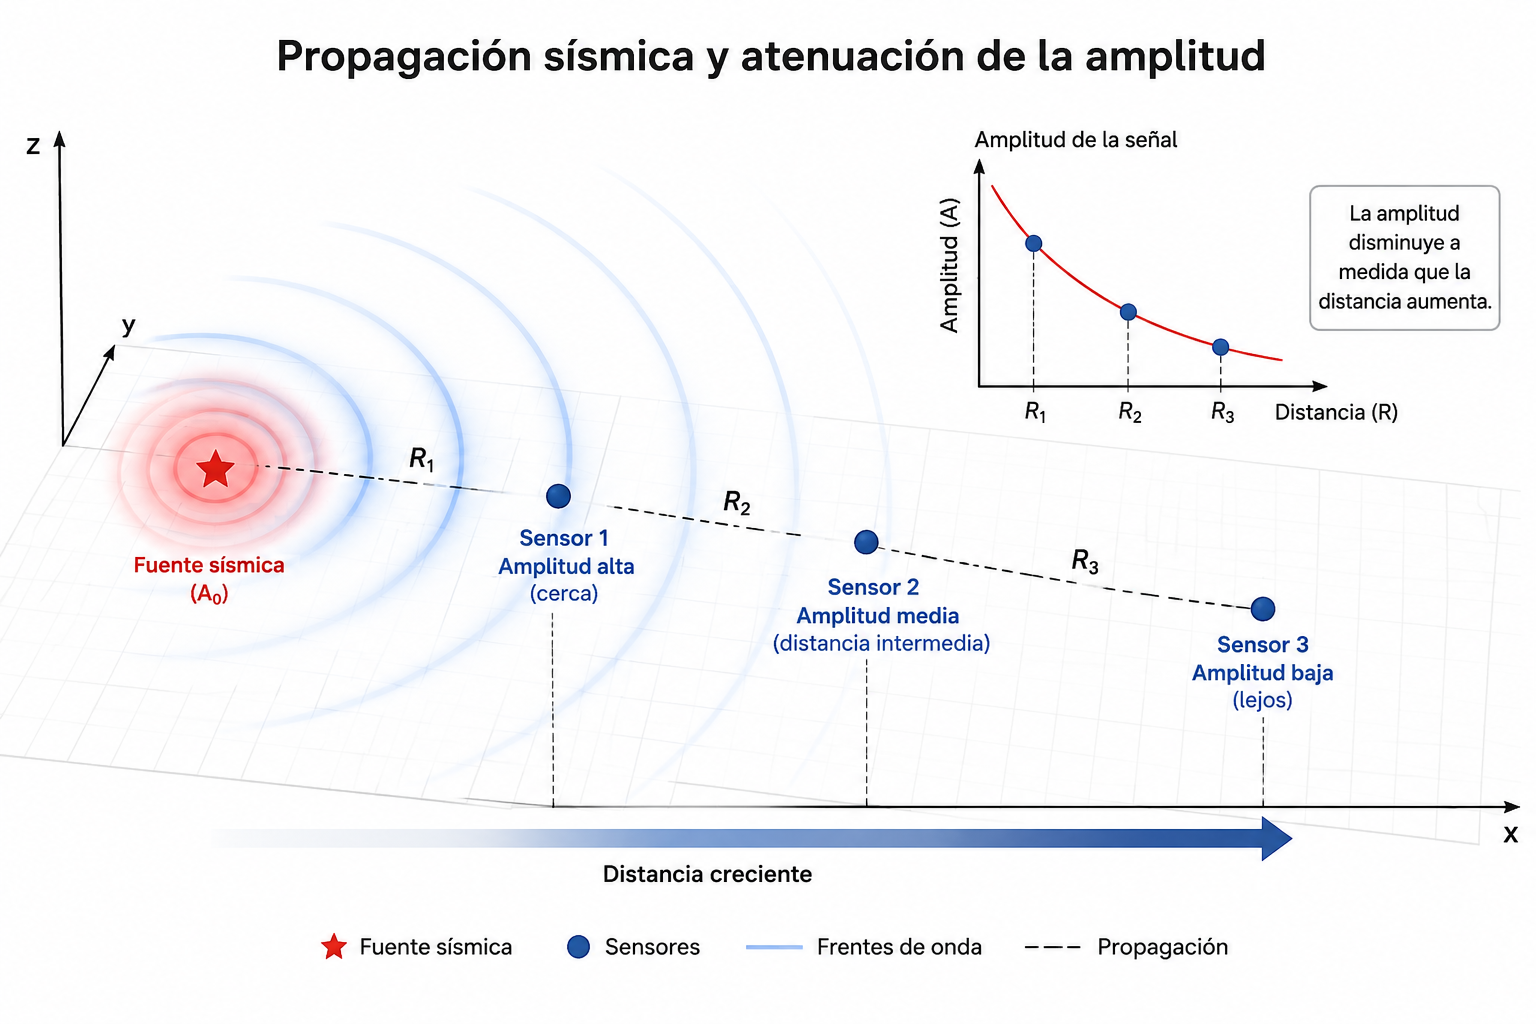
\includegraphics[width=0.80\textwidth]{Imagenes/PropagaciónSísmicaAtenuaciónAmplitud.png}
            
            \vspace{0.2cm}
            
            % Pequeño resumen del flujo por si Kevin necesita apoyarse al hablar
            \scriptsize
            Fuente Sísmica $\rightarrow$ Propagación $\rightarrow$ Pérdida de energía
        \end{center}
    
        % PARTE DERECHA: Significado de cada componente
        \column{0.48\textwidth}
        % Bajamos un poco el texto para que quede centrado respecto a la imagen
        \vspace{0.3cm} 
        
        \small
        \begin{itemize}
            \item $A_0$ : amplitud inicial de la fuente.
            \vspace{0.3cm} % Espacio extra entre items para mayor legibilidad
            
            \item $e^{-R_i}$ : atenuación de energía durante la propagación.
            \vspace{0.3cm}
            
            \item $\frac{1}{R_i}$ : dispersión geométrica de la onda.
            \vspace{0.3cm}
            
            \item $R_i$ : distancia entre la fuente y el sensor.
        \end{itemize}
        
    \end{columns}
    
    \vspace{0.4cm}
    
    % PARTE INFERIOR: Frase clave
    \begin{center}
        \textbf{
            La amplitud disminuye a medida que aumenta la \\ distancia entre la fuente y el sensor.
        }
    \end{center}

\end{frame}